\section{Les filtres de convolution}
Pour pouvoir faire la squeletisation de l'image nous avons eu besoin de faire des filtres de convolution pour pouvoir faire un filtre laplaciene et ainsi detourer l'ensemble de charactere en vu de les extraire. Nous allons donc expliquer comment se met un place un filtre de convolution.
\subsection{l'avantage}
L'avantage des filtres de convolution est qu'il s'agit d'un seul et même algorithme pour plusieur filtre. En effet l'algorithme prend en paramètre une image et une matrice de 3x3 ou 5x5 et applique à tout les composantes de chaque pixel la formule suivante :
\begin{center}
\[x_{11} = \sum_{i=0}^2\sum_{j=0}^2 \lambda_{ij} \times x_{ij}\]
où $x_{ij}$ est le pixel correspondant a la cellule de matrice $\lambda_{ij}$
\end{center}
\subsection{le filtre laplacien}
Nous avons utiliser un fitre laplacien car il nous permet de detourer les charactère rendant ainsi l'extraction bien plus facile.
Le filtre laplacien est caractérisé par la matrice 
\begin{center}
\[ \left(
  \begin{array}{ c c c }
     0 & 1  & 0\\
     1 & -4 & 1\\
     0 & 1  & 0
  \end{array} \right)
\]
\end{center}
Il s'agit donc d'un filtre rehausseur autrement dit, un filtre passe haut.
Le resultat est ensuite diviser par 9 pour obtenir un élément linéaire.
\begin{center}
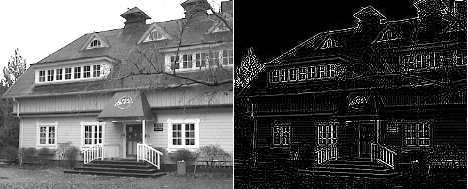
\includegraphics{conv-laplacian-result.png}
\end{center}
Nous Pouvons aussi revenir a notre filtre media. Il s'agit aussi d'un filtre de convolution avec la matrice mais d'un filtre passe-bas car il permet d'augmenter la netteter de l'image.
